% Rascunho da seção de resultados. Texto final com a equipe.
% Requer % Gerado por src/analysis/artigo_tex.py a partir de results/. Não edite à mão.
\newcommand{\bandaQuatroCinco}{1,7}
\newcommand{\bandaQuatroQuinze}{5,2}
\newcommand{\bandaQuatroTrinta}{10,5}
\newcommand{\bandaSeisCinco}{3,0}
\newcommand{\bandaSeisQuinze}{8,9}
\newcommand{\bandaSeisTrinta}{17,7}
\newcommand{\bandaTresCinco}{0,8}
\newcommand{\bandaTresQuinze}{2,5}
\newcommand{\bandaTresTrinta}{5,0}
\newcommand{\etoeSsdFpQuatroNuvem}{102}
\newcommand{\etoeSsdFpTresNuvem}{87}
\newcommand{\etoeYoloFpQuatroNuvem}{111}
\newcommand{\etoeYoloFpSeisNuvem}{165}
\newcommand{\etoeYoloFpTresNuvem}{77}
\newcommand{\mapSsdFpQuatroNuvem}{0,595}
\newcommand{\mapSsdFpTresNuvem}{0,592}
\newcommand{\mapYoloFpQuatroNuvem}{0,745}
\newcommand{\mapYoloFpSeisNuvem}{0,761}
\newcommand{\mapYoloFpTresNuvem}{0,668}
\newcommand{\nCenarios}{15}
\newcommand{\nCombBorda}{0}
\newcommand{\nCombNuvem}{5}
\newcommand{\nQuadrosValidos}{300}
 no preâmbulo e as tabelas de docs/artigo/tabelas/ (geradas por e6).
% Todos os valores vêm das macros: se a coleta for refeita, rode e6 e o texto acompanha.
\section{Resultados}
\label{sec:resultados}

Foram medidas \nCombBorda{} combinações na borda e \nCombNuvem{} na nuvem, com \nQuadrosValidos{}
quadros válidos cada, das quais se derivaram \nCenarios{} cenários de taxa da fonte. Os tempos de borda
foram obtidos em ARM64 nativo (servidor Neoverse-N1, 2 núcleos) e são usados em comparações relativas.

\subsection{Qualidade da detecção}
A Tabela~\ref{tab:qualidade} mostra o mAP@50 da classe pessoa. O YOLOv8n teve a melhor qualidade e é o
único que melhora com a resolução (\mapYoloFpTres{}, \mapYoloFpQuatro{} e \mapYoloFpSeis{} em FP32 a 320,
480 e 640), porque é o único modelo cuja entrada acompanha a resolução da fonte; no SSD-MobileNet~V1
(\mapSsdFpTres{}) e no EfficientDet-Lite0 (\mapEffdetFpTres{}) a resolução da fonte quase não altera o
resultado, já que o quadro é reduzido para a entrada fixa. A quantização INT8 custou pouca qualidade: no
YOLOv8n a 640 o mAP@50 passou de \mapYoloFpSeis{} para \mapYoloIntSeis{}, no EfficientDet-Lite0 a 320 de
\mapEffdetFpTres{} para \mapEffdetIntTres{}, e no SSD-MobileNet~V1 a variação ficou dentro de
centésimos (\mapSsdFpTres{} e \mapSsdIntTres{} a 320).

% Gerado por src/analysis/artigo_tex.py. Não edite à mão.
\begin{table}[htbp]
\centering
\scriptsize
\setlength{\tabcolsep}{3pt}
\caption{Qualidade da detecção de pessoas (mAP@50 e F1 com limiar 0,5) nas 350 imagens do COCO val2017.}
\label{tab:qualidade}
\begin{tabular}{llllrr}
\hline
Parte & Modelo & Precisão & Resolução & mAP@50 & F1 \\
\hline
borda & YOLOv8n & FP32 & 320 & 0,679 & 0,602 \\
borda & YOLOv8n & FP32 & 480 & 0,750 & 0,668 \\
borda & YOLOv8n & FP32 & 640 & 0,770 & 0,690 \\
borda & YOLOv8n & INT8 & 320 & 0,676 & 0,599 \\
borda & YOLOv8n & INT8 & 480 & 0,744 & 0,645 \\
borda & YOLOv8n & INT8 & 640 & 0,760 & 0,671 \\
borda & SSD-MobileNet V1 & FP32 & 320 & 0,603 & 0,595 \\
borda & SSD-MobileNet V1 & FP32 & 480 & 0,603 & 0,601 \\
borda & SSD-MobileNet V1 & FP32 & 640 & 0,602 & 0,603 \\
borda & SSD-MobileNet V1 & INT8 & 320 & 0,605 & 0,603 \\
borda & SSD-MobileNet V1 & INT8 & 480 & 0,605 & 0,611 \\
borda & SSD-MobileNet V1 & INT8 & 640 & 0,610 & 0,611 \\
borda & EfficientDet-Lite0 & FP32 & 320 & 0,514 & 0,519 \\
borda & EfficientDet-Lite0 & FP32 & 480 & 0,512 & 0,517 \\
borda & EfficientDet-Lite0 & FP32 & 640 & 0,507 & 0,516 \\
borda & EfficientDet-Lite0 & INT8 & 320 & 0,472 & 0,502 \\
borda & EfficientDet-Lite0 & INT8 & 480 & 0,468 & 0,495 \\
borda & EfficientDet-Lite0 & INT8 & 640 & 0,469 & 0,492 \\
nuvem & YOLOv8n & FP32 & 320 & 0,668 & 0,591 \\
nuvem & YOLOv8n & FP32 & 480 & 0,745 & 0,653 \\
nuvem & YOLOv8n & FP32 & 640 & 0,761 & 0,680 \\
nuvem & SSD-MobileNet V1 & FP32 & 320 & 0,592 & 0,555 \\
nuvem & SSD-MobileNet V1 & FP32 & 480 & 0,595 & 0,583 \\
nuvem & SSD-MobileNet V1 & FP32 & 640 & 0,600 & 0,583 \\
nuvem & EfficientDet-Lite0 & FP32 & 320 & 0,506 & 0,511 \\
nuvem & EfficientDet-Lite0 & FP32 & 480 & 0,512 & 0,521 \\
nuvem & EfficientDet-Lite0 & FP32 & 640 & 0,498 & 0,507 \\
\hline
\end{tabular}
\end{table}


\subsection{Desempenho na borda (QP1)}
A Tabela~\ref{tab:latencia_borda} resume a latência fim a fim por quadro. A quantização INT8 reduziu a
latência em todas as combinações, com diferença significativa em todos os pares
(Tabela~\ref{tab:testes_fp32_int8}): o ganho foi de cerca de \razaoYoloTres{} vezes no YOLOv8n,
\razaoSsdTres{} no SSD-MobileNet~V1 e \razaoEffdetTres{} no EfficientDet-Lite0 (fonte de 320). No YOLOv8n a
latência cresce com a resolução (\etoeYoloIntTres{}, \etoeYoloIntQuatro{} e \etoeYoloIntSeis{}\,ms em INT8),
enquanto nos modelos de entrada fixa só o custo de redimensionar o quadro aumenta. O processo ocupou
quase os dois núcleos durante a inferência (por exemplo, \cpuYoloFpSeis\% no YOLOv8n FP32 a 640) e usou
entre \rssYoloIntTres{} e \rssYoloFpSeis{}\,MB de memória residente no YOLOv8n, descontados os quadros
pré-carregados.

Nos cenários derivados, o YOLOv8n FP32 a 640 sustenta \fpsYoloFpSeis{} quadros por segundo: a 15 e a 30
FPS a fila cresce continuamente e uma política de descarte perderia \descYoloFpSeisQuinze\% e
\descYoloFpSeisTrinta\% dos quadros. Em INT8, todas as combinações sustentam 30 FPS, exceto o YOLOv8n a
640 (\fpsYoloIntSeis{} FPS). Em FP32, SSD-MobileNet~V1 e EfficientDet-Lite0 sustentam 15 FPS, mas não 30
(Figura~\ref{fig:descarte}). Como o núcleo Neoverse-N1 é mais rápido que o do Raspberry Pi~4, esses
limites devem ser lidos como relativos: a ordem entre modelos e precisões é o que se espera transferir
para a placa.

% Gerado por src/analysis/artigo_tex.py. Não edite à mão.
\begin{table}[htbp]
\centering
\footnotesize
\caption{Latência fim a fim por quadro na borda (s; média e IC 95\%), ambiente emulado (QEMU, perfil rpi4b).}
\label{tab:latencia_borda}
\begin{tabular}{llccr}
\hline
Modelo & Resolução & FP32 & INT8 & FP32/INT8 \\
\hline
YOLOv8n & 320 & -- & 4,00 [3,95; 4,05] & -- \\
YOLOv8n & 480 & -- & 8,14 [8,04; 8,23] & -- \\
\hline
\end{tabular}
\par\smallskip\parbox{0.95\linewidth}{\scriptsize Tempos medidos em emulação: servem para comparação relativa, não representam um Raspberry Pi. 300 quadros válidos por combinação.}
\end{table}

% Gerado por src/analysis/artigo_tex.py. Não edite à mão.
\begin{table}[htbp]
\centering
\footnotesize
\caption{Testes pareados da latência fim a fim FP32 $\times$ INT8 na borda (Shapiro-Wilk nas diferenças; $\alpha = 0{,}05$).}
\label{tab:testes_fp32_int8}
\begin{tabular}{llrrlr}
\hline
Modelo & Res. & Pares & Shapiro $p$ & Teste & $p$ \\
\hline
\multicolumn{6}{c}{(sem dados)} \\
\hline
\end{tabular}
\end{table}


\subsection{Acelerador Edge TPU}
Sem o acelerador físico, avaliou-se a compilação (Tabela~\ref{tab:edgetpu}). Só o SSD-MobileNet~V1 INT8
compilou, com todas as operações mapeadas para a TPU e o modelo inteiro cabendo na memória do chip. O
YOLOv8n INT8 foi recusado por não ser inteiramente quantizado (entrada e saída em float32) e o
EfficientDet-Lite0 INT8 falhou em um operador de soma. Na prática, só o SSD-MobileNet~V1 se beneficiaria
do acelerador sem mudanças no modelo.

% Gerado por src/analysis/artigo_tex.py. Não edite à mão.
\begin{table}[htbp]
\centering
\footnotesize
\caption{Compilação dos modelos INT8 para o Edge TPU (edgetpu\_compiler 14.1).}
\label{tab:edgetpu}
\begin{tabular}{llcrrl}
\hline
Modelo & Res. & Compilou & Op. na TPU & Op. total & Memória no chip \\
\hline
EfficientDet-Lite0 & 320 & não & -- & -- & -- \\
SSD-MobileNet V1 & 300 & sim & 64 & 64 & 6.99MiB \\
YOLOv8n & 320 & não & -- & -- & -- \\
YOLOv8n & 480 & não & -- & -- & -- \\
YOLOv8n & 640 & não & -- & -- & -- \\
\hline
\end{tabular}
\end{table}


\subsection{Borda $\times$ nuvem (QP2)}
No baseline de nuvem (Tabela~\ref{tab:nuvem}), cada quadro JPEG exige banda de subida que cresce com a
resolução e a taxa da fonte: a 15 FPS são \bandaTresQuinze{}, \bandaQuatroQuinze{} e
\bandaSeisQuinze{}\,Mbit/s a 320, 480 e 640, e a 30 FPS o quadro de 640 pixels exigiria
\bandaSeisTrinta{}\,Mbit/s, acima do enlace de subida emulado (10\,Mbit/s). Na borda nenhum quadro de
vídeo sai do dispositivo, só o resultado da detecção (Figura~\ref{fig:banda}). Este é o resultado
principal da QP2. A latência fim a fim da nuvem (\etoeYoloFpTresNuvem{} a \etoeYoloFpSeisNuvem{}\,ms
no YOLOv8n) inclui a transmissão do quadro, que domina o tempo nas resoluções maiores; ela não é
comparada em valor absoluto com a da borda, porque os dois lados rodaram em servidores diferentes e
nenhum deles é um Raspberry Pi.

% Gerado por src/analysis/artigo_tex.py a partir de results/. Não edite à mão.
\begin{table*}[t]
\centering
\footnotesize
\caption{Baseline de nuvem: latência média por quadro, tamanho do quadro JPEG e banda de subida demandada por taxa da câmera.}
\label{tab:nuvem}
\setlength{\tabcolsep}{4pt}
\begin{tabular}{@{}llrrrr*{3}{r}@{}}
\toprule
& & \multicolumn{3}{c}{Latência média (ms)} & & \multicolumn{3}{c}{Banda de subida (Mbit/s)} \\ \cmidrule(lr){3-5} \cmidrule(l){7-9}
Modelo & {Res. (px)} & {fim a fim} & {transm.} & {infer.} & {kB/quadro} & {5 FPS} & {15 FPS} & {30 FPS} \\
\midrule
YOLOv8n & 320 & 77 & 38 & 16 & 20,7 & 0,8 & 2,5 & 5,0 \\
 & 480 & 111 & 57 & 27 & 43,6 & 1,7 & 5,2 & 10,5 \\
 & 640 & 165 & 82 & 52 & 73,9 & 3,0 & 8,9 & 17,7 \\
SSD-MobileNet V1 & 320 & 87 & 38 & 19 & 20,7 & 0,8 & 2,5 & 5,0 \\
 & 480 & 102 & 57 & 13 & 43,6 & 1,7 & 5,2 & 10,5 \\
 & 640 & 136 & 83 & 17 & 73,9 & 3,0 & 8,9 & 17,7 \\
EfficientDet-Lite0 & 320 & 91 & 38 & 25 & 20,7 & 0,8 & 2,5 & 5,0 \\
 & 480 & 106 & 57 & 17 & 43,6 & 1,7 & 5,2 & 10,5 \\
 & 640 & 137 & 82 & 19 & 73,9 & 3,0 & 8,9 & 17,7 \\
\bottomrule
\end{tabular}
\par\smallskip
\parbox{0.96\linewidth}{\scriptsize Servidor x86-64 nativo, modelos FP32; enlace emulado com tc netem (RTT 40 ms, subida 10 Mbit/s). A banda demandada independe do enlace. Na borda nenhum quadro de vídeo é enviado.}
\end{table*}


\begin{figure}[htbp]
\centering
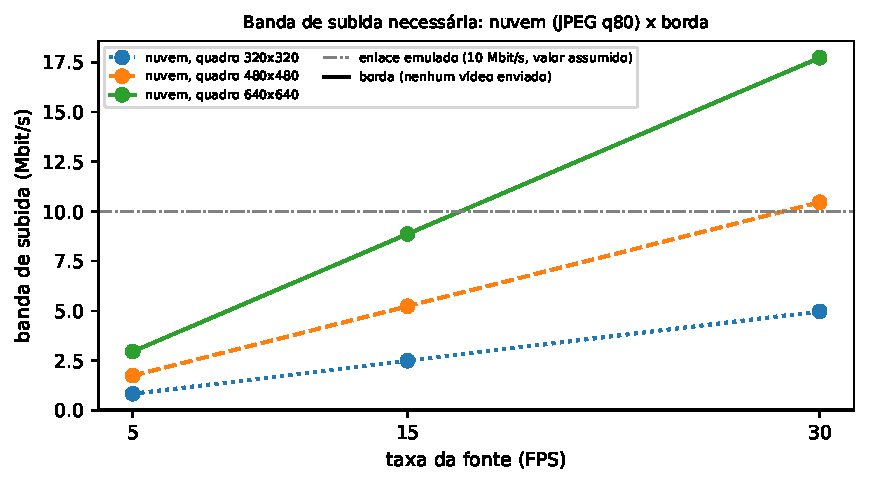
\includegraphics[width=0.85\linewidth]{../../figures/e6_banda_subida.pdf}
\caption{Banda de subida necessária para enviar o vídeo à nuvem (JPEG qualidade 80) em função da taxa
e da resolução da fonte, comparada à borda, que não envia vídeo.}
\label{fig:banda}
\end{figure}

\begin{figure}[htbp]
\centering
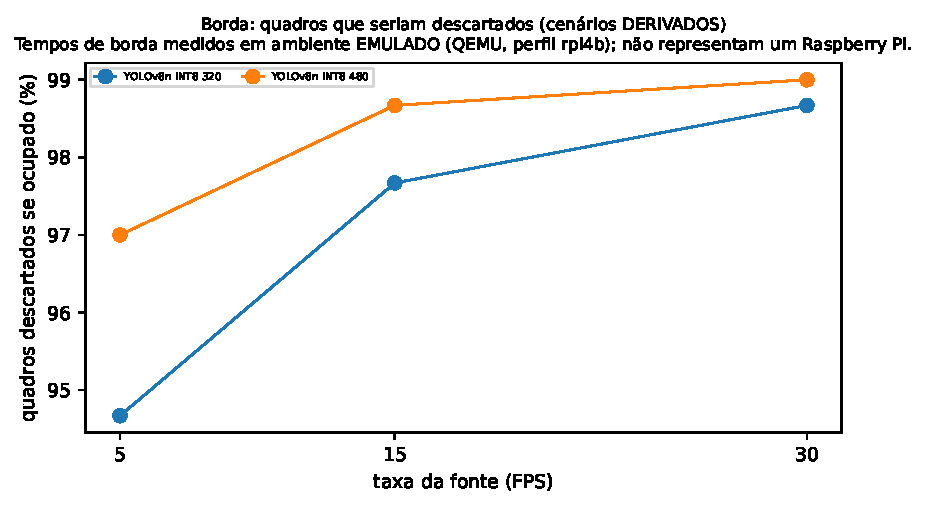
\includegraphics[width=0.85\linewidth]{../../figures/e6_borda_descarte.pdf}
\caption{Quadros que seriam descartados na borda com a política de processar o quadro mais recente
(cenários derivados, ARM64 nativo com 2 núcleos).}
\label{fig:descarte}
\end{figure}
